\documentclass[12pt,a4paper]{article}

% --- Metadata ---
\def\courseshortheader{HỌC MÁY ỨNG DỤNG --- HỒI QUY TUYẾN TÍNH}
\def\coverbookline{TRÍ TUỆ NHÂN TẠO}
\def\covermaintitle{Hồi quy tuyến tính}
\def\coversubtitle{Lý thuyết --- Mất mát, tham số, gradient descent, siêu tham số}

% Shared preamble for nhom_5 (requires \courseshortheader before \input)
\usepackage[utf8]{inputenc}
\usepackage[vietnamese]{babel}
\usepackage{amsmath,amssymb,amsthm}
\usepackage{geometry}
\usepackage{enumitem}
\usepackage[most]{tcolorbox}
\usepackage{hyperref}
\usepackage{fancyhdr}
\usepackage{graphicx}
\usepackage{booktabs}
\usepackage{tikz}
\usetikzlibrary{calc,arrows.meta,decorations.pathreplacing,positioning}
\usepackage{eso-pic}
\usepackage{xcolor}

\geometry{a4paper, margin=2cm, bottom=2.5cm}
\hypersetup{colorlinks=true, linkcolor=blue!70!black, urlcolor=blue}
\setlist[itemize]{topsep=4pt, itemsep=2pt}
\setlist[enumerate]{topsep=4pt, itemsep=2pt}

\AddToShipoutPictureFG{%
  \AtPageCenter{%
    \begin{tikzpicture}[remember picture, overlay]
      \node[rotate=45, scale=1, opacity=0.06]{%
        \fontsize{60}{72}\selectfont\bfseries\sffamily Đặng Tấn Quí%
      };
    \end{tikzpicture}%
  }%
}

\pagestyle{fancy}
\fancyhf{}
\fancyhead[L]{\small\textit{\courseshortheader}}
\fancyhead[R]{\small\textit{Đặng Tấn Quí}}
\fancyfoot[C]{\thepage}
\fancyfoot[L]{\footnotesize\textcopyright\ Đặng Tấn Quí}
\fancyfoot[R]{\footnotesize SĐT: 0377\,122\,210}
\renewcommand{\headrulewidth}{0.4pt}
\renewcommand{\footrulewidth}{0.4pt}

\fancypagestyle{plain}{%
  \fancyhf{}
  \fancyfoot[C]{\thepage}
  \fancyfoot[L]{\footnotesize\textcopyright\ Đặng Tấn Quí}
  \fancyfoot[R]{\footnotesize SĐT: 0377\,122\,210}
  \renewcommand{\headrulewidth}{0pt}
  \renewcommand{\footrulewidth}{0.4pt}
}

\newtcolorbox{dongco}[1][]{%
  enhanced, breakable,
  colback=teal!4!white, colframe=teal!60!black,
  fonttitle=\bfseries, title={Động cơ học -- Tại sao cần khái niệm này?}, #1%
}
\newtcolorbox{ynghia}[1][]{%
  enhanced, breakable,
  colback=purple!3!white, colframe=purple!50!black,
  fonttitle=\bfseries, title={Ý nghĩa \& Trực giác}, #1%
}
\newtcolorbox{ungdung}[1][]{%
  enhanced, breakable,
  colback=olive!5!white, colframe=olive!60!black,
  fonttitle=\bfseries, title={Ứng dụng thực tế}, #1%
}
\newtcolorbox{dinhnghia}[1][]{%
  enhanced, breakable,
  colback=blue!3!white, colframe=blue!60!black,
  fonttitle=\bfseries, title={Định nghĩa}, #1%
}
\newtcolorbox{dinhly}[1][]{%
  enhanced, breakable,
  colback=green!3!white, colframe=green!50!black,
  fonttitle=\bfseries, title={Định lý}, #1%
}
\newtcolorbox{tinhchat}[1][]{%
  enhanced, breakable,
  colback=yellow!5!white, colframe=orange!50!black,
  fonttitle=\bfseries, title={Tính chất}, #1%
}
\newtcolorbox{phuongphap}[1][]{%
  enhanced, breakable,
  colback=gray!5!white, colframe=gray!50!black,
  fonttitle=\bfseries, title={Phương pháp}, #1%
}
\newtcolorbox{luuy}[1][]{%
  enhanced, breakable,
  colback=red!3!white, colframe=red!50!black,
  fonttitle=\bfseries, title={Lưu ý}, #1%
}
\newtcolorbox{congthuc}[1][]{%
  enhanced, breakable,
  colback=cyan!3!white, colframe=cyan!50!black,
  fonttitle=\bfseries, title={Công thức}, #1%
}
\newtcolorbox{vidu}[1][]{%
  enhanced, breakable,
  colback=violet!3!white, colframe=violet!50!black,
  fonttitle=\bfseries, title={Ví dụ}, #1%
}
\newtcolorbox{phanvidu}[1][]{%
  enhanced, breakable,
  colback=red!2!white, colframe=red!40!black,
  fonttitle=\bfseries, title={Phản ví dụ}, #1%
}
\newtcolorbox{tongket}[1][]{%
  enhanced, breakable,
  colback=blue!4!white, colframe=blue!70!black,
  fonttitle=\bfseries, title={Tổng kết chương}, #1%
}


\usepackage{tabularx}
\usepackage{array}
\usepackage{float}
\usepackage{amsmath}

\graphicspath{{images/linear-regression/}}

\newcommand{\mlimg}[2][0.88]{\begin{center}\includegraphics[width=#1\linewidth]{#2}\end{center}}

\begin{document}

\thispagestyle{empty}
\begin{tikzpicture}[remember picture, overlay]
  \fill[blue!80!black] (current page.south west) rectangle (current page.north east);
  \fill[blue!60!cyan, opacity=0.8]
    (current page.south west) -- (current page.north west) --
    ([xshift=-3cm]current page.north east) -- (current page.south east) -- cycle;
  \foreach \r/\o in {6/0.05, 4.5/0.08, 3/0.12} {
    \fill[white, opacity=\o] ([xshift=2cm, yshift=-2cm]current page.north east) circle (\r cm);
  }
  \draw[white, line width=2pt] ([yshift=-5cm]current page.north west) ++(2cm,0) -- ++(17cm,0);
  \draw[white, line width=2pt] ([yshift=-16cm]current page.north west) ++(2cm,0) -- ++(17cm,0);
  \node[anchor=west, white, font=\fontsize{28}{34}\bfseries\selectfont]
    at ([xshift=3cm, yshift=-7.5cm]current page.north west) {\coverbookline};
  \node[anchor=west, white, font=\fontsize{20}{26}\selectfont]
    at ([xshift=3cm, yshift=-9cm]current page.north west) {\covermaintitle};
  \node[anchor=west, white, font=\fontsize{16}{22}\selectfont]
    at ([xshift=3cm, yshift=-10.2cm]current page.north west) {\coversubtitle};
  \node[anchor=west, white, font=\Large\bfseries]
    at ([xshift=3cm, yshift=-13cm]current page.north west) {Biên soạn:};
  \node[anchor=west, yellow!80!white, font=\fontsize{24}{30}\bfseries\selectfont]
    at ([xshift=3cm, yshift=-14.5cm]current page.north west) {ĐẶNG TẤN QUÍ};
  \node[anchor=west, white!90, font=\large]
    at ([xshift=3cm, yshift=-18cm]current page.north west) {SĐT: 0377\,122\,210};
  \node[anchor=south, white!80, font=\small]
    at ([yshift=1.5cm]current page.south) {Tài liệu có bản quyền --- Cấm sao chép khi chưa được sự đồng ý của tác giả};
  \node[anchor=south east, white, font=\Large\bfseries]
    at ([xshift=-2cm, yshift=3cm]current page.south east) {\the\year};
\end{tikzpicture}

\newpage
\tableofcontents
\newpage

\section*{Lời nói đầu}
\addcontentsline{toc}{section}{Lời nói đầu}

\begin{ynghia}[title={Nguồn và cách đọc}]
Tài liệu biên soạn và dịch từ \emph{Linear Regression} (Google ML Crash Course)\footnote{\url{https://developers.google.com/machine-learning/crash-course/linear-regression}}.
\end{ynghia}

\begin{luuy}[title={Điều kiện tiên quyết}]
Cần nắm khái niệm từ \href{https://developers.google.com/machine-learning/intro-to-ml}{Introduction to Machine Learning}: mẫu, đặc trưng, nhãn, huấn luyện, mất mát, hồi quy có giám sát.
\end{luuy}

\begin{phuongphap}[title={Mục tiêu học tập}]
\begin{itemize}
  \item Giải thích hàm mất mát và cách dùng trong huấn luyện.
  \item Mô tả gradient descent tìm tham số tối ưu (trọng số, bias).
  \item Điều chỉnh siêu tham số (learning rate, batch size, epoch) để huấn luyện hiệu quả.
\end{itemize}
\end{phuongphap}

\newpage

%==============================================================================
\section{Hồi quy tuyến tính (linear regression)}
%==============================================================================

\begin{dongco}[title={Dự đoán mức tiêu thụ nhiên liệu}]
Cho biết \textbf{trọng lượng xe} (nghìn pound), ta muốn dự đoán \textbf{dặm/gallon} (MPG). Quan hệ gần \textbf{tuyến tính}: xe nặng hơn $\Rightarrow$ MPG thường thấp hơn. Hồi quy tuyến tính tìm đường thẳng (hoặc siêu phẳng) ``khớp'' dữ liệu nhất.
\end{dongco}

\begin{dinhnghia}[title={Hồi quy tuyến tính}]
\href{https://developers.google.com/machine-learning/glossary\#linear-regression}{Hồi quy tuyến tính} tìm quan hệ giữa
\href{https://developers.google.com/machine-learning/glossary\#feature}{đặc trưng} và
\href{https://developers.google.com/machine-learning/glossary\#label}{nhãn}. Trong ML, đó là mô hình dự đoán nhãn số từ đặc trưng bằng tổ hợp \textbf{tuyến tính} của các đặc trưng.
\end{dinhnghia}

\begin{vidu}[title={Dữ liệu mẫu --- Trọng lượng vs MPG}]
\begin{center}
\small
\begin{tabular}{cc}
\textbf{Trọng lượng (nghìn pound)} & \textbf{MPG (nhãn)} \\
\midrule
3.5 & 18 \\
3.69 & 15 \\
3.44 & 18 \\
3.43 & 16 \\
4.34 & 15 \\
4.42 & 14 \\
2.37 & 24 \\
\end{tabular}
\end{center}
\end{vidu}

\mlimg{car-data-points.png}
\begin{center}\small\textbf{Hình 1.} Trọng lượng vs MPG --- xu hướng giảm.\end{center}

Khi ô tô càng nặng, chỉ số quãng đường đi được trên một gallon nhiên liệu thường giảm.

\mlimg{car-data-points-with-model.png}
\begin{center}\small\textbf{Hình 2.} Đường khớp tốt nhất (best fit).\end{center}

\subsection{Phương trình hồi quy tuyến tính}

\begin{congthuc}[title={Dạng đại số và dạng ML (một đặc trưng)}]
Đại số: $y = mx + b$ với $y$ = MPG, $x$ = trọng lượng, $m$ = độ dốc, $b$ = giao $Oy$.

\medskip
ML (một đặc trưng):
\[
  y' = b + w_1 x_1
\]
\begin{itemize}
  \item $y'$: nhãn \textbf{dự đoán}.
  \item $b$: \href{https://developers.google.com/machine-learning/glossary\#bias-math-or-bias-term}{\textbf{bias}} (tương đương $w_0$, giao $Oy$ - tung độ gốc) --- tham số học được.
  \item $w_1$: \href{https://developers.google.com/machine-learning/glossary\#weight}{\textbf{trọng số}} (tương đương độ dốc - hệ số góc $m$) --- tham số học được.
  \item $x_1$: đặc trưng đầu vào (không đổi trong tập dữ liệu).
\end{itemize}
\end{congthuc}

\mlimg[0.75]{equation.png}
\begin{center}\small\textbf{Hình 3.} Các thành phần phương trình.\end{center}

\begin{vidu}[title={Đọc tham số từ đường khớp}]
Từ đồ thị: $b \approx 34$, $w_1 \approx -4{,}6$.
\[
  y' = 34 + (-4{,}6)\, x_1
\]
Xe 4{,}000 pound ($x_1 = 4$): Dự đoán MPG $\approx 15{,}6$.
\end{vidu}

\mlimg[0.85]{model-prediction.png}
\begin{center}\small\textbf{Hình 4.} Dự đoán tại $x_1 = 4$.\end{center}

\subsection{Mô hình nhiều đặc trưng}

\begin{congthuc}[title={Nhiều đặc trưng}]
\[
  y' = b + w_1 x_1 + w_2 x_2 + \cdots + w_n x_n
\]
Ví dụ dự đoán MPG thêm: dung tích xi-lanh, gia tốc, số xi-lanh, mã lực.
\end{congthuc}

\mlimg[0.7]{equation-multiple-features.png}
\begin{center}\small\textbf{Hình 5.} Phương trình năm đặc trưng.\end{center}

\mlimg[0.75]{displacement.png}
\begin{center}\small\textbf{Hình 6.} Dung tích xi-lanh vs MPG (quan hệ tuyến tính âm).\end{center}

\mlimg[0.75]{acceleration.png}
\begin{center}\small\textbf{Hình 7.} Gia tốc vs MPG (quan hệ tuyến tính dương).\end{center}

\begin{tinhchat}[title={Phần nào được cập nhật khi huấn luyện?}]
\begin{itemize}
  \item \textbf{Cập nhật:} bias $b$ và các trọng số $w_i$.
  \item \textbf{Không cập nhật:} $y'$ (là kết quả tính), giá trị đặc trưng $x_i$ (cố định trong dataset).
\end{itemize}
\end{tinhchat}

\newpage

%==============================================================================
\section{Mất mát (loss)}
%==============================================================================

\begin{dongco}[title={Làm sao biết đường thẳng ``tốt''?}]
Hai đường khác nhau đều ``nhìn ổn'' trên đồ thị MPG --- cần một \textbf{số} đo mức sai.
\end{dongco}

\begin{dinhnghia}[title={Mất mát}]
  \href{https://developers.google.com/machine-learning/glossary\#loss}{\textbf{Mất mát}} (loss) đo khoảng cách giữa dự đoán $y'$ và nhãn thật $y$; mục tiêu huấn luyện là \textbf{giảm mất mát} tới mức thấp nhất có thể. Mất mát (loss) không quan tâm dự đoán \textbf{cao hơn} hay \textbf{thấp hơn}, chỉ quan tâm \textbf{xa bao nhiêu}.
\end{dinhnghia}

\mlimg[0.85]{loss-lines.png}
\begin{center}\small\textbf{Hình 8.} Mũi tên loss: từ giá trị thực tới dự đoán.\end{center}

\begin{ynghia}[title={Bỏ dấu khi tính loss}]
Dự đoán 2, thực tế 5: sai $-3$ nhưng ta chỉ cần \textbf{khoảng cách 3} chứ không cần hướng.

Hai cách phổ biến:
\begin{itemize}
  \item \textbf{Trị tuyệt đối} $|y - y'|$;
  \item \textbf{Bình phương} $(y - y')^2$.
\end{itemize}
\end{ynghia}

\begin{dinhnghia}[title={Năm loại mất mát thường gặp}]
\begin{tabularx}{\textwidth}{@{}>{\raggedright\arraybackslash}p{4.8cm} X >{\raggedright\arraybackslash}p{4.8cm}@{}}
\textbf{Loại} & \textbf{Ý nghĩa} & \textbf{Công thức} \\
\midrule
$L_1$ loss &
Tổng $|y - y'|$ trên các mẫu &
$\displaystyle\sum |y - y'|$ \\
Sai số trung bình tuyệt đối (MAE) &
Trung bình $L_1$ trên $N$ mẫu &
$\dfrac{1}{N}\displaystyle\sum |y - y'|$ \\
$L_2$ loss &
Tổng $(y - y')^2$ &
$\displaystyle\sum (y - y')^2$ \\
Sai số bình phương trung bình (MSE) &
Trung bình $L_2$ trên $N$ mẫu &
$\dfrac{1}{N}\displaystyle\sum (y - y')^2$ \\
Căn bậc hai của sai số bình phương trung bình (RMSE) &
Căn bậc hai của MSE (cùng thang với $y$) &
$\sqrt{\text{MSE}}$ \\
\end{tabularx}
\end{dinhnghia}

\begin{tinhchat}[title={$L_1$ vs $L_2$ --- ảnh hưởng của bình phương}]
\begin{itemize}
  \item Sai số \textbf{lớn}: bình phương làm loss \textbf{càng lớn thêm}.
  \item Sai số \textbf{nhỏ} ($< 1$): bình phương làm loss \textbf{nhỏ hơn nữa}.
  \item MAE/RMSE thường \textbf{dễ diễn giải} hơn (cùng đơn vị với nhãn); RMSE nhạy hơn với lỗi lớn so với MAE.
\end{itemize}
\end{tinhchat}

\begin{luuy}
Khi xử lý nhiều mẫu, nên \textbf{lấy trung bình} (MAE, MSE, RMSE) thay vì chỉ cộng tổng $L_1$/$L_2$ thuần.
\end{luuy}

\begin{vidu}[title={Vi dụ: Tính $L_2$ loss cho một điểm}]
Mô hình MPG: $y' = 34 + (-4{,}6)\, x_1$

Xe 2{,}370 pound ($x_1 = 2{,}37$ nghìn pound): dự đoán $y' \approx 23{,}1$ MPG, thực tế $y = 24$ MPG.
\[
  L_2 = (24 - 23{,}1)^2 = 0{,}81
\]
\end{vidu}

\begin{ynghia}[title={Ngoại lệ (outlier) trong dữ liệu và trong dự đoán}]
\textbf{Outlier dữ liệu:} xe 8{,}000 pound hoặc 100 MPG --- ngoài khoảng thường (2--5 nghìn pound, 8--50 MPG).

\textbf{Outlier dự đoán:} xe 3{,}000 pound, 40 MPG có thể hợp lý trong dữ liệu nhưng mô hình dự đoán $\sim$20 MPG --- lệch lớn so với thực tế.
\end{ynghia}

\begin{phuongphap}[title={Khi nào dùng MSE / RMSE? Khi nào dùng MAE?}]
\textbf{Chọn MSE (hoặc RMSE) khi:}
\begin{itemize}
  \item Muốn \textbf{phạt nặng} sai số lớn.
  \item Coi outlier là phản ánh biến thiên thật mà mô hình nên học.
  \item Cần tối ưu ``mượt'' (tính chất toán của MSE thuận lợi cho gradient descent).
\end{itemize}

\textbf{Chọn MAE khi:}
\begin{itemize}
  \item Dataset có outlier mà không muốn chúng \textbf{kéo} mô hình quá mạnh.
  \item Muốn loss = ``sai số trung bình'' dễ hiểu trực tiếp.
\end{itemize}

\medskip
Thực tế còn phụ thuộc \textbf{bài toán kinh doanh}: loại sai lệch nào ``đắt'' hơn.
\end{phuongphap}

\mlimg[0.8]{model-mse.png}
\begin{center}\small\textbf{Hình 9.} Huấn luyện với MSE --- đường (đỏ) gần outlier hơn.\end{center}

\mlimg[0.8]{model-mae.png}
\begin{center}\small\textbf{Hình 10.} Huấn luyện với MAE --- đường xa outlier, gần đám đông hơn.\end{center}

\begin{tinhchat}[title={So sánh trực quan}]
\begin{itemize}
  \item \textbf{MSE:} mô hình gần outlier, xa phần lớn điểm còn lại.
  \item \textbf{MAE:} mô hình xa outlier, gần phần lớn điểm.
\end{itemize}
\end{tinhchat}

\begin{luuy}[title={MSE trên hai đồ thị}]
\begin{center}
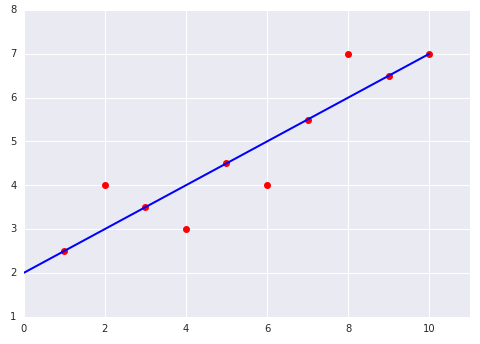
\includegraphics[width=0.44\linewidth]{mse-left.png}\hfill
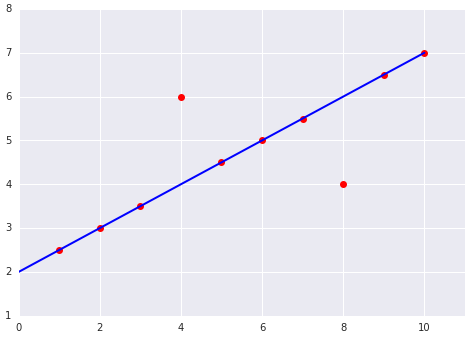
\includegraphics[width=0.44\linewidth]{mse-right.png}

\small\textbf{Hình 11.} Trái \hspace{2cm} \textbf{Hình 12.} Phải
\end{center}
\textbf{Đồ thị bên phải} có MSE cao hơn ($\approx 0{,}8$ vs $\approx 0{,}4$): nhiều điểm trên đường nhưng hai điểm lệch \textbf{gấp đôi} khoảng cách; bình phương làm loss tăng mạnh ($2^2 = 4$ lần so với lệch 1).
\end{luuy}

\begin{phanvidu}
MSE = 0 trên mọi điểm $\Rightarrow$ khớp hoàn hảo --- thường là \textbf{overfitting}, không phải mục tiêu thực tế.
\end{phanvidu}

\newpage

%==============================================================================
\section{Bài tập về tham số}
%==============================================================================

\begin{phuongphap}[title={Nhiệm vụ (Parameters exercise)}]
\begin{enumerate}
  \item Vẽ 20 mẫu: trục $x$ = trọng lượng (nghìn pound), trục $y$ = MPG.
  \item Điều chỉnh Weight và Bias để tìm đường thẳng \textbf{minimize MSE}.
  \item Ghi MSE thấp nhất và cặp $(w, b)$ tương ứng.
\end{enumerate}
Link bài tập: https://developers.google.com/machine-learning/crash-course/linear-regression/parameters-exercise
\end{phuongphap}

\begin{vidu}[title={Đáp án}]
MSE tối thiểu $\approx 3{,}37$ với $w = -0{,}12$, $b = 16{,}96$.
\end{vidu}

\mlimg[0.85]{parameters-exercise-solution.png}
\begin{center}\small\textbf{Hình 13.} Đường tối ưu cho bài tập tham số.\end{center}

\begin{ynghia}
\textbf{Tham số} ($w$, $b$) quyết định độ nghiêng và vị trí đường;

\textbf{MSE} đo tổng bình phương sai số --- gradient descent tự làm việc này.
\end{ynghia}

\newpage

%==============================================================================
\section{Phương pháp giảm độ dốc (gradient descent)}
%==============================================================================

\begin{dongco}[title={Không thể thử hết mọi $(w,b)$}]
Với hai tham số còn tìm được bằng mắt; với hàng chục đặc trưng thì không. \href{https://developers.google.com/machine-learning/glossary\#gradient-descent}{\textbf{Gradient descent}} (GD) lặp: tính mất mát $\to$ biết hướng giảm $\to$ bước nhỏ $\to$ lặp đến \textbf{hội tụ}.

Video: \url{https://www.youtube.com/watch?v=QoK1nNAURw4}
\end{dongco}

\begin{dinhnghia}[title={Gradient descent}]
Kỹ thuật lặp tìm $w$, $b$ (và các tham số khác) sao cho \textbf{mất mát} (thường MSE) \textbf{nhỏ nhất}.
\end{dinhnghia}

\begin{phuongphap}[title={Vòng lặp gradient descent}]
\begin{enumerate}
  \item Khởi tạo $w$, $b$ gần 0 (ngẫu nhiên nhỏ).
  \item Tính mất mát với $w$, $b$ hiện tại.
  \item Tính hướng (gradient) làm \textbf{giảm} mất mát.
  \item Cập nhật $w$, $b$ một bước nhỏ theo hướng đó.
  \item Lặp đến khi không giảm thêm đáng kể (\textbf{hội tụ}).
\end{enumerate}
\end{phuongphap}

\mlimg[0.9]{gradient-descent.png}
\begin{center}\small\textbf{Hình 14.} Quy trình gradient descent.\end{center}

\subsection{MSE và bước tính cụ thể}

\begin{congthuc}[title={MSE (Mean Squared Error)}]
Với $M$ mẫu, dự đoán $f_{w,b}(x) = wx + b$, nhãn thật $y$:
\[
  \text{MSE} = \dfrac{1}{M}\displaystyle\sum_{i=1}^{M}\bigl(f_{w,b}(x^{(i)}) - y^{(i)}\bigr)^2
\]
\end{congthuc}

\begin{vidu}[title={7 mẫu dữ liệu}]
  \begin{center}
  \begin{tabular}{cc}
    \textbf{Pao (tính bằng nghìn)} & \textbf{Số dặm trên mỗi ga lông (nhãn)} \\
    \midrule
    3,5 & 18 \\
    3,69 & 15 \\
    3,44 & 18 \\
    3,43 & 16 \\
    4,34 & 15 \\
    4,42 & 14 \\
    2,37 & 24 \\
  \end{tabular}
  \end{center}
\end{vidu}

\begin{phuongphap}[title={Khởi tạo $w=0$, $b=0$ và tính MSE}]
\begin{enumerate}
  \item MSE = $\dfrac{1}{7}\displaystyle\sum_{i=1}^{7}\bigl(0 - y^{(i)}\bigr)^2 \approx 303{,}71$ (dự đoán 0 cho mọi mẫu).
  \item Đạo hàm theo $w$: độ dốc tiếp tuyến $\dfrac{\partial}{\partial w}\text{MSE} \approx -119{,}7$; theo $b$: $\dfrac{\partial}{\partial b}\text{MSE} \approx -34{,}3$.
  \item Bước nhỏ $\eta = 0{,}01$ (learning rate):
  \[
    w_{\text{mới}} = w_{\text{cũ}} - \eta x \dfrac{\partial}{\partial w}\text{MSE} = 0 - 0{,}01 \times (-119{,}7) \approx 1{,}2,\quad
    b_{\text{mới}} = b_{\text{cũ}} - \eta x \dfrac{\partial}{\partial b}\text{MSE} = 0 - 0{,}01 \times (-34{,}3) \approx 0{,}34
  \]
\end{enumerate}
\end{phuongphap}

\begin{congthuc}[title={Đạo hàm MSE}]
\[
  \dfrac{\partial}{\partial w}\text{MSE}
  = \dfrac{1}{M}\displaystyle\sum_{i=1}^{M} 2\bigl(f_{w,b}(x^{(i)}) - y^{(i)}\bigr)\, x^{(i)}
\]
\[
  \dfrac{\partial}{\partial b}\text{MSE}
  = \dfrac{1}{M}\displaystyle\sum_{i=1}^{M} 2\bigl(f_{w,b}(x^{(i)}) - y^{(i)}\bigr)
\]
Gradient âm $\Rightarrow$ tăng $w$, $b$ để giảm mất mát (với khởi tạo 0).
\end{congthuc}

\begin{table}[H]
\centering
\caption{MSE giảm qua các vòng lặp (ví dụ minh họa)}
\begin{tabular}{cccc}
\textbf{Vòng} & \textbf{Weight} & \textbf{Bias} & \textbf{MSE} \\
\midrule
1 & 0 & 0 & 303.71 \\
2 & 1.20 & 0.34 & 170.84 \\
3 & 2.05 & 0.59 & 103.17 \\
4 & 2.66 & 0.78 & 68.70 \\
5 & 3.09 & 0.91 & 51.13 \\
6 & 3.40 & 1.01 & 42.17 \\
\end{tabular}
\end{table}

\begin{luuy}[title={Hội tụ và huấn luyện quá lâu}]
Khi \href{https://developers.google.com/machine-learning/glossary\#convergence}{hội tụ}, thêm vòng lặp hầu như không giảm MSE; huấn luyện thêm có thể làm mất mát \textbf{dao động nhẹ} quanh cực tiểu. Cần theo dõi đến khi mất mát \textbf{ổn định}.
\end{luuy}

\subsection{Đường cong mất mát và hội tụ}

\begin{ynghia}[title={Loss curve}]
\href{https://developers.google.com/machine-learning/glossary\#loss-curve}{Đường cong mất mát}: trục $y$ = loss, trục $x$ = số vòng lặp. Giảm mạnh đầu, sau đó phẳng dần $\Rightarrow$ mô hình đã hội tụ.
\end{ynghia}

\mlimg[0.8]{convergence.png}
\begin{center}\small\textbf{Hình 15.} Hội tụ quanh vòng $\sim$1000.\end{center}

\mlimg[0.72]{large-loss.png}
\begin{center}\small\textbf{Hình 16.} Đầu huấn luyện --- loss lớn.\end{center}

\mlimg[0.72]{med-loss.png}
\begin{center}\small\textbf{Hình 17.} Giữa quá trình --- đường gần dữ liệu hơn.\end{center}

\mlimg[0.72]{low-loss.png}
\begin{center}\small\textbf{Hình 18.} Cuối --- loss thấp, đường khớp tốt.\end{center}

\begin{luuy}
\textbf{Vai trò GD:} lặp tìm $w$, $b$ \textbf{minimize loss}. GD \textbf{không} chọn loại loss (L1/L2) và \textbf{không} xóa outlier khỏi dataset.
\end{luuy}

\subsection{Hàm lồi và cực tiểu toàn cục}

\begin{dinhly}[title={Mô hình tuyến tính và hàm lồi}]
Mất mát của hồi quy tuyến tính tạo mặt \href{https://developers.google.com/machine-learning/glossary\#convex-function}{\textbf{lồi}} (convex). Khi hội tụ, mô hình đã tìm $(w,b)$ cho \textbf{mất mát thấp nhất} (cực tiểu toàn cục).
\end{dinhly}

\mlimg[0.75]{convexity.png}
\begin{center}\small\textbf{Hình 19.} Mặt mất mát lồi.\end{center}

\mlimg[0.75]{loss-weight-bias.png}
\begin{center}\small\textbf{Hình 20.} Cực tiểu: $w \approx -5{,}44$, $b \approx 35{,}94$, MSE $\approx 5{,}54$.\end{center}

\begin{ynghia}[title={Quả bóng lăn xuống đồi}]
Các điểm $(w,b)$ trong GD như quả bóng lăn xuống đáy thung lũng mất mát; thực tế thường đạt \textbf{gần} cực tiểu.
\end{ynghia}

\mlimg[0.75]{loss-surface-points.png}
\begin{center}\small\textbf{Hình 21.} Điểm GD trên mặt loss.\end{center}

\mlimg[0.85]{graphed-model.png}
\begin{center}\small\textbf{Hình 22.} Mô hình với $w$, $b$ tối ưu.\end{center}

\begin{phanvidu}[title={MSE = 0 không phải lúc nào cũng tốt}]
MSE = 0 nghĩa là khớp \textbf{mọi} điểm --- thường là \textbf{overfitting}. Cực tiểu thực tế thường $> 0$.
\end{phanvidu}

\newpage

%==============================================================================
\section{Siêu tham số (hyperparameters)}
%==============================================================================

\begin{dongco}[title={Ai điều khiển tốc độ học?}]
\textbf{Tham số} ($w$, $b$) do mô hình học.

\textbf{Siêu tham số} do \textbf{người} đặt trước: learning rate, batch size, số epoch --- quyết định \emph{cách} và \emph{tốc độ} hội tụ.
\end{dongco}

\begin{tinhchat}[title={Siêu tham số vs tham số}]
\begin{itemize}
  \item \textbf{Siêu tham số} (\href{https://developers.google.com/machine-learning/glossary\#hyperparameter}{hyperparameter}): learning rate, batch size, epochs --- bạn kiểm soát.
  \item \textbf{Tham số} (\href{https://developers.google.com/machine-learning/glossary\#parameter}{parameter}): $w$, $b$ --- mô hình tính khi huấn luyện.
\end{itemize}
\end{tinhchat}

\subsection{Tốc độ học (learning rate)}

\begin{dinhnghia}[title={Tốc độ học}]
  Tốc độ học xác định mức độ thay đổi cần thực hiện đối với các trọng số và độ lệch trong mỗi bước của quy trình hạ độ dốc, ảnh hưởng đến tốc độ hội tụ của mô hình. Nếu tốc độ học quá thấp, mô hình có thể mất nhiều thời gian để hội tụ. Tuy nhiên, nếu tốc độ học tập quá cao, mô hình sẽ không bao giờ hội tụ, mà thay vào đó sẽ dao động xung quanh các trọng số và độ lệch giúp giảm thiểu tổn thất. Mục tiêu là chọn tốc độ học tập không quá cao cũng không quá thấp để mô hình hội tụ nhanh chóng.
  
  Hệ số $\eta$ nhân với gradient để quyết định \textbf{độ lớn bước} cập nhật $w$, $b$ mỗi vòng. Sự khác biệt giữa các tham số mô hình cũ và các tham số mô hình mới tỷ lệ thuận với độ dốc của hàm tổn thất. Ví dụ: nếu độ dốc lớn, mô hình sẽ thực hiện một bước lớn. Nếu nhỏ, hãy thực hiện một bước nhỏ.
  
  Trong ví dụ GD trước, ``bước nhỏ'' $0{,}01$ chính là learning rate.
\end{dinhnghia}

\begin{congthuc}[title={Cập nhật với learning rate}]
\[
  w_{\text{mới}} = w_{\text{cũ}} - \eta \cdot \dfrac{\partial \text{MSE}}{\partial w},\qquad
  b_{\text{mới}} = b_{\text{cũ}} - \eta \cdot \dfrac{\partial \text{MSE}}{\partial b}
\]
Gradient lớn $\Rightarrow$ bước lớn (nếu $\eta$ cố định); gradient nhỏ $\Rightarrow$ bước nhỏ.
\end{congthuc}

\begin{dinhnghia}[title={Learning rate và đường cong mất mát}]
\begin{tabularx}{\textwidth}{@{}l X@{}}
\textbf{Mức} & \textbf{Hiện tượng} \\
\midrule
Phù hợp & Giảm nhanh rồi phẳng --- hội tụ trong số vòng hợp lý. \\
Quá nhỏ & Cải thiện chậm từng vòng --- cần rất nhiều vòng. \\
Quá lớn & Loss dao động hoặc tăng --- không hội tụ. \\
\end{tabularx}
\end{dinhnghia}

\mlimg[0.75]{correct-lr.png}
\begin{center}\small\textbf{Hình 23.} Learning rate tốt.\end{center}

\mlimg[0.75]{small-lr.png}
\begin{center}\small\textbf{Hình 24.} Learning rate quá nhỏ.\end{center}

\mlimg[0.75]{high-lr.png}
\begin{center}\small\textbf{Hình 25.} Learning rate quá lớn --- dao động.\end{center}

\mlimg[0.75]{increasing-loss.png}
\begin{center}\small\textbf{Hình 26.} Learning rate quá lớn --- loss tăng.\end{center}

\begin{luuy}
Learning rate \textbf{lý tưởng phụ thuộc bài toán} --- không có một số cố định (0.01 hay 1.0) cho mọi dataset.
\end{luuy}

\subsection{Batch size}

\begin{dinhnghia}[title={Batch size}]
Số \href{https://developers.google.com/machine-learning/glossary\#example}{mẫu} xử lý trong mỗi lần huấn luyện trước khi tiến hành cập nhật $w$, $b$.

Cách hoạt động: Thay vì đưa toàn bộ tập dữ liệu khổng lồ vào huấn luyện cùng lúc (gây tràn bộ nhớ) hoặc đưa từng mẫu một (tốn thời gian), dữ liệu được chia thành các lô nhỏ (mini-batch). Batch size chính là số lượng mẫu trong mỗi lô đó.

Ví dụ: Bạn có tập dữ liệu 1000 ảnh. Nếu bạn chọn batch size = 32, mô hình sẽ lấy 32 ảnh đầu tiên để học, điều chỉnh hệ số, sau đó lấy tiếp 32 ảnh tiếp theo, v.v.

Huấn luyện AI giống như một người đang cố gắng đi xuống đáy của một thung lũng (điểm hội tụ/tối ưu) trong điều kiện sương mù dày đặc.

Tăng Batch Size (Gộp nhiều dữ liệu hơn trong mỗi bước): Giống như việc người đi bộ dừng lại, quan sát kỹ một nhóm cột mốc (thay vì chỉ nhìn một cột mốc nhỏ lẻ) trước khi quyết định hướng đi. Quá trình này giúp mô hình "nhìn" tổng quát dữ liệu nhanh hơn trong mỗi epoch, từ đó đưa ra bước đi chính xác, vững chắc và bớt chệch hướng.
\end{dinhnghia}

\begin{tinhchat}[title={Ba kiểu cập nhật}]
\begin{itemize}
  \item \textbf{Giảm độ dốc ngẫu nhiên trên toàn bộ batch (Full batch)}: toàn dataset $\to$ 1 cập nhật / epoch. Tuy nhiên, khi dataset chứa hàng trăm nghìn hoặc thậm chí hàng triệu mẫu, việc sử dụng toàn bộ batch là không thực tế.
  \item \textbf{Giảm độ dốc ngẫu nhiên (SGD)}: 1 mẫu / bước --- nhanh, \textbf{nhiễu} (loss nhấp nhô).
  \item \textbf{Giảm độ dốc ngẫu nhiên trên batch nhỏ (Mini-batch SGD)}: $1 < \text{batch} < N$ --- cân bằng; gradient trung bình trên batch.
\end{itemize}
\end{tinhchat}

\mlimg[0.75]{noisy-gradient.png}
\begin{center}\small\textbf{Hình 27.} SGD --- nhiễu trên loss curve.\end{center}

\mlimg[0.75]{mini-batch-sgd.png}
\begin{center}\small\textbf{Hình 28.} Mini-batch --- ít nhiễu hơn gần hội tụ.\end{center}

\begin{ynghia}[title={Nhiễu không luôn xấu}]
Một mức nhiễu có thể giúp \href{https://developers.google.com/machine-learning/glossary\#generalization}{tổng quát hóa} tốt hơn và tìm ra các trọng số và độ lệch tối ưu trong một \href{https://developers.google.com/machine-learning/glossary?hl=vi#neural-network}{mạng nơ-ron}.
\end{ynghia}

\subsection{Epoch}

\begin{dinhnghia}[title={Epoch}]
Một \href{https://developers.google.com/machine-learning/glossary\#epoch}{epoch} = mô hình đã duyệt \textbf{toàn bộ} tập huấn luyện đúng một lần. Ví dụ: 1000 mẫu, batch 100 $\Rightarrow$ 10 lần lặp (\href{https://developers.google.com/machine-learning/glossary\#iteration}{iteration}) trong mỗi epoch.
\end{dinhnghia}

\mlimg[0.85]{batch-size.png}
\begin{center}\small\textbf{Hình 29.} Full batch, mini-batch, epoch.\end{center}

\begin{congthuc}[title={Số lần cập nhật tham số (ví dụ 1000 mẫu, 20 epoch)}]
\begin{tabularx}{\textwidth}{@{}l X@{}}
\textbf{Kiểu batch} & \textbf{Cập nhật $w$, $b$} \\
\midrule
Full batch & 20 lần (1 lần / epoch, hình dung 1 batch x 20 epoch). \\
SGD & 20\,000 lần (1 mẫu / epoch, hình dung 1\,000 batch x 20 epoch ). \\
Mini-batch (100) & 200 lần (10 batch $\times$ 20 epoch). \\
\end{tabularx}
\end{congthuc}

\begin{luuy}
\begin{enumerate}
  \item Batch size mini-batch \textbf{tùy dataset và tài nguyên}, không cố định 10 hay 100.
  \item Tăng gấp đôi learning rate có thể làm huấn luyện \textbf{chậm hơn} (nhảy quá mạnh, không hội tụ).
  \item Batch lớn ``không phù hợp'' dữ liệu nhiều outlier --- trung bình gradient trên batch lớn có thể \textbf{giảm} ảnh hưởng outlier.
\end{enumerate}
\end{luuy}

\newpage

%==============================================================================
\section{Bài tập về phương pháp giảm độ dốc}
%==============================================================================

\begin{dongco}[title={Thực hành learning rate}]
Cùng dữ liệu MPG, lần này máy tự chạy GD. Ba mức learning rate cho ba kiểu hành vi: hội tụ nhanh, quá chậm, không hội tụ.

Link bài tập: https://developers.google.com/machine-learning/crash-course/linear-regression/gradient-descent-exercise
\end{dongco}

\begin{phuongphap}[title={Ba nhiệm vụ}]
\begin{description}
  \item[Nhiệm vụ 1:] Learning rate $= 0{,}03$, nhấn Start. Ghi thời gian hội tụ, MSE, $w$, $b$.
  \item[Nhiệm vụ 2:] Reset; learning rate $\approx 1{,}1 \times 10^{-5}$. Quan sát tốc độ hội tụ.
  \item[Nhiệm vụ 3:] Reset; learning rate $= 1$. Quan sát loss dao động / không hội tụ.
\end{description}
\end{phuongphap}

\begin{vidu}[title={Đáp án nhiệm vụ 1}]
$\eta = 0{,}03$: hội tụ $\sim$30 giây; MSE $\approx 2{,}67$; $w \approx -1{,}14$, $b \approx 20{,}389$ --- learning rate hợp lý.
\end{vidu}

\begin{vidu}[title={Đáp án nhiệm vụ 2}]
$\eta \approx 10^{-5}$: sau vài phút vẫn chưa hội tụ; mỗi bước giảm loss rất ít $\Rightarrow$ nên \textbf{tăng} learning rate.
\end{vidu}

\begin{vidu}[title={Đáp án nhiệm vụ 3}]
$\eta = 1$: MSE nhảy mạnh (có thể $> 300$), dao động --- \textbf{quá lớn}, không bao giờ hội tụ ổn định.
\end{vidu}

\begin{tongket}[title={Tổng kết chương --- Hồi quy tuyến tính}]
\begin{itemize}
  \item Mô hình: $y' = b + \displaystyle\sum_i w_i x_i$; học $w$, $b$ bằng cách giảm MSE.
  \item \textbf{Gradient descent:} lặp tính gradient và cập nhật; mặt loss lồi $\Rightarrow$ cực tiểu tin cậy.
  \item \textbf{Siêu tham số:} $\eta$ (learning rate), batch size, epoch --- cần thử nghiệm theo dataset.
\end{itemize}
\end{tongket}

\end{document}
